\section{Introduction}
\label{sec:intro}

    \begin{frame}
    \frametitle{Introduction and Problem Statement}
    \begin{itemize}
        \item The increasing frequency of wildfires has led to a demand for \textbf{automated monitoring systems}.
        \item Traditional methods (satellites, thermal sensors) suffer from \textbf{delayed data retrieval}.
        \item \textbf{Deep learning} techniques can be used to \textbf{improve detection speed and accuracy}.
    \end{itemize}

    \begin{figure}
        \centering
        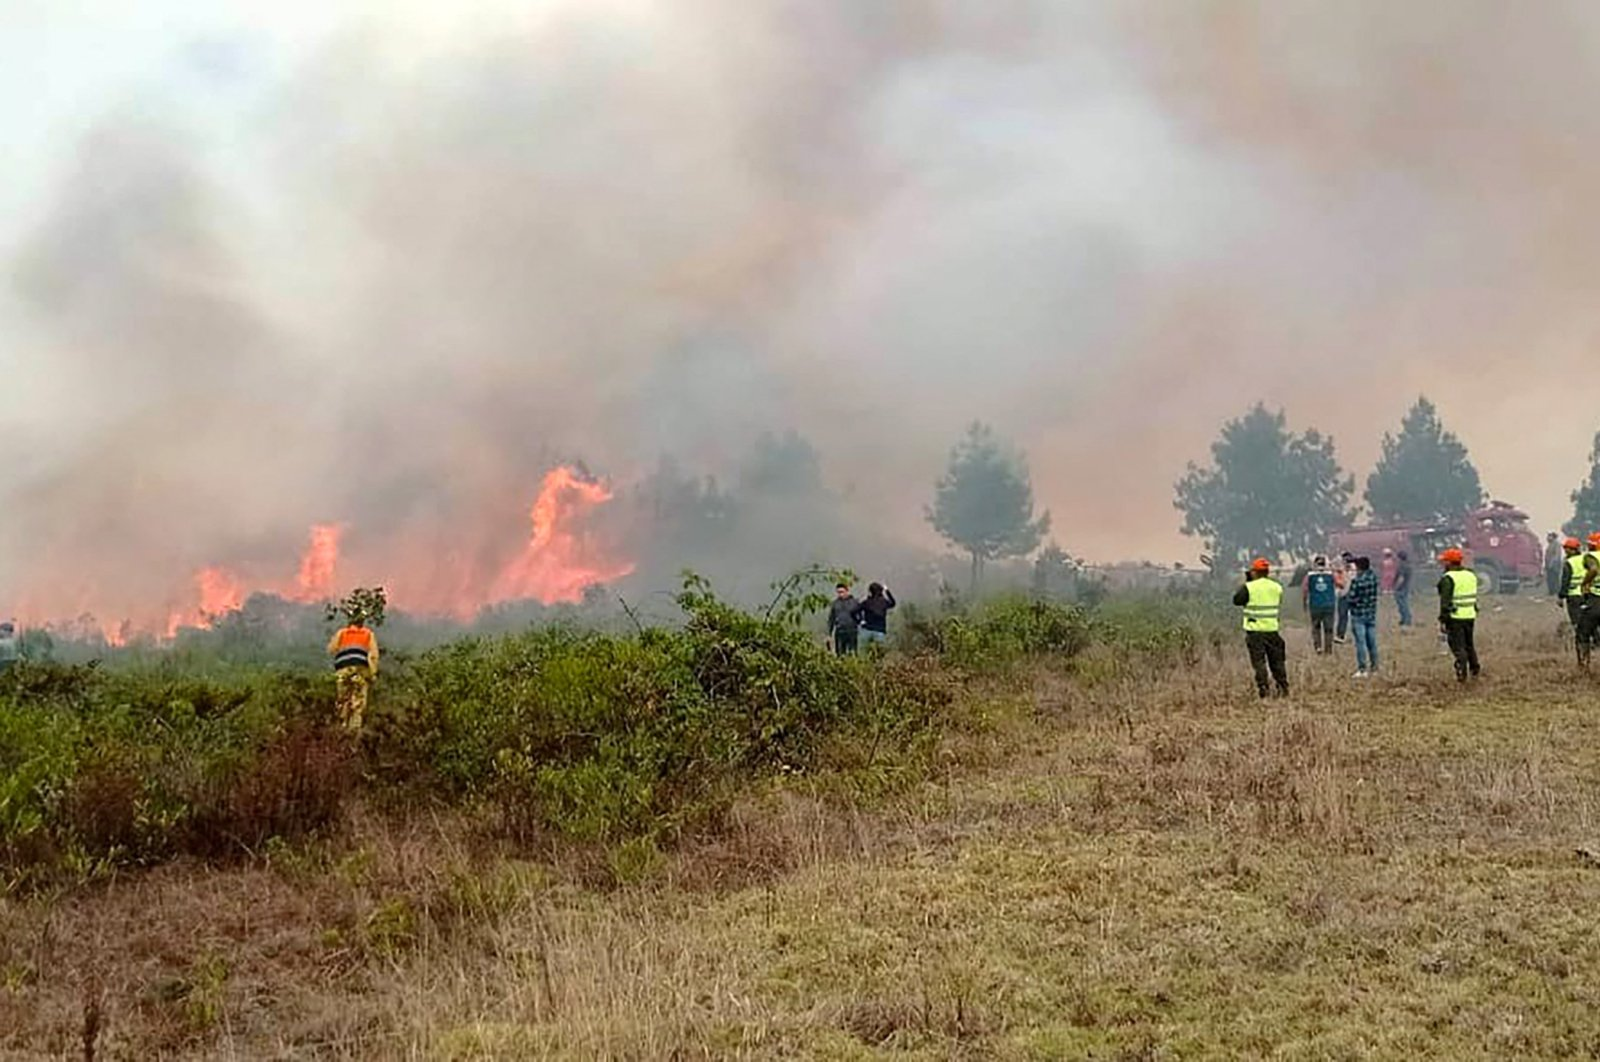
\includegraphics[width=0.4\textwidth]{images/wildfire}
        \caption{Wildfire in Peru. Source: \textit{Daily Sabah}}
        \label{fig:wildfire}
    \end{figure}
\end{frame}

\begin{frame}
    \frametitle{Research Motivation and Goals}
    \blocky{Objective of this Study}{
        \begin{itemize}
            \item Develop an \textbf{ensemble of CNNs} for \textbf{wildfire detection} in aerial images.
            \item Evaluate the performance of \textbf{Xception, DenseNet121, and ResNet152}.
            \item Improve classification accuracy while keeping computational efficiency.
        \end{itemize}
    }
\end{frame}